%%%%%%%%%%%%%%%%%%%%%%%%%%%%%%%%%%%%%%%%%%%%%%%%%%%%%%%%%%%%%%%%%%%%%%%%
% Plantilla TFG/TFM
% Escuela Politécnica Superior de la Universidad de Alicante
% Realizado por: Jose Manuel Requena Plens
% Contacto: info@jmrplens.com / Telegram:@jmrplens
%%%%%%%%%%%%%%%%%%%%%%%%%%%%%%%%%%%%%%%%%%%%%%%%%%%%%%%%%%%%%%%%%%%%%%%%
\chapter{Resultados}
\label{resultados}
En este apartado usaré comparaciones en gráficas para ver claramente las ventajas y/o inconvenientes de algunas decisiones que he tomado durante el desarrollo de este proyecto.

\section{Optimización de caché}
Como he mencionado en el desarrollo, el motor \gls{ecs} está pensado para ser ``cache-friendly''. Esto quiere decir que la memoria del programa se organiza de tal manera que optimiza la caché. Esto sucede, como ya he comentado, porque la caché lee streams de memoria, y no solo un dato. Por lo tanto, merece la pena tener los datos que vayamos a utilizar en el juego ordenados en memoria, de esta manera el juego podrá realizar más acciones por frame, debido a que la velocidad de un acceso a memoria en caché es, aproximadamente, 200 veces más rápida que un acceso a memoria RAM.

Mi primera idea para demostrar esto fue hacer un test en el cual tienes un vector de tamaño ``3x'', y tres vectores de tamaño ``x''. Supuestamente el vector del triple de tamaño conseguirá mayor velocidad al leer la memoria de forma lineal, mientras que será más lento realizar lecturas de los tres vectores, ya que el acceso a la memoria no será lineal.
\begin{lstlisting}[style=C-color, caption={Caché optimizada vs sin optimizar. Primer intento},label=cache-optimization-first]
	size_t bench_optimized(const std::vector<int>& the_one, size_t times) {
		size_t result = 0;
		
		for(std::size_t i=0; i<times; ++i) {
			for (std::size_t j = 0; j < the_one.size(); j++) {
				result += the_one[j];
			}
		}
		
		return result;
	}
	size_t bench_unoptimized(const std::vector<int>& first, const std::vector<int>& second, const std::vector<int>& third, size_t times) {
		size_t result = 0;
		
		for(std::size_t i=0; i<times; ++i) {
			for (std::size_t j = 0; j < first.size(); j++) {
				result += first[j];
				result += second[j];
				result += third[j];
			}
		}
		
		return result;
	}
\end{lstlisting}

Los resultados de este test son que el que supuestamente debería ser más lento, tarda menos tiempo en ejecutarse. Esto puede ser porque el procesador tiene varias lineas de caché, o también porque los procesadores modernos tienen instrucciones \gls{simd}, lo que hace que se puedan realizar las tres sumas de golpe y eso también explicaría una ejecución más rápida del test.
\begin{figure}[H]
	\centering
	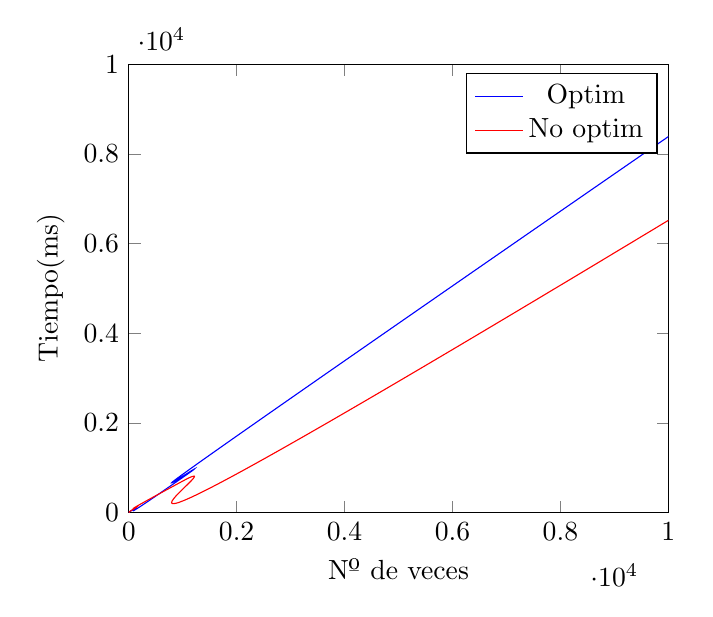
\begin{tikzpicture}
		\begin{axis}
			[ymin=0,ymax=10000, 
			xmin=0,xmax=10000, 
			ylabel= Tiempo(ms), 
			xlabel= Nº de veces] 
			\addplot+[smooth, mark=none] coordinates 
			{(1,1) (10,12) (100,82) (1000,782) (10000,8385) (100000,83121)};
			\addplot+[smooth, mark=none] coordinates
			{(1,0) (10,7) (100,83) (1000,701) (10000,6517) (100000,72598)};
			\legend{Optim, No optim}
		\end{axis}
	\end{tikzpicture}
	\caption{Comparación de optimización vs sin optimización. Primer intento.}
\end{figure}

El siguiente ejemplo que se me ocurrió fue el típico problema de orden de lectura de datos de una matriz. He simplificado un ejemplo con el cual demostrar que el orden en el que se lee la memoria es importante. El siguiente código es una matriz, la cual se lee primero de manera "cache-friendly", y después no.
\begin{lstlisting}[style=C-color, caption={Caché optimizada vs sin optimizar. Segundo intento},label=cache-optimization-second]
size_t bench_optimized(size_t v[][width], size_t times) {
	size_t result = 0;
	
	for(size_t i=0; i<times; ++i) {
		for (size_t j = 0; j < height; ++j) 
			for (size_t k = 0; k < width; ++k)
				result += v[j][k];
	}
	
	return result;
}
size_t bench_unoptimized(size_t v[][width], size_t times) {
	size_t result = 0;
	
	for(size_t i=0; i<times; ++i) {
		for (size_t k = 0; k < width; ++k) 
			for (size_t j = 0; j < height; ++j) 
				result += v[j][k];
	}
	
	return result;
}
\end{lstlisting}

La diferencia en ambos métodos está en los dos for anidados. Una vez programados los dos métodos, procedo a hacer una comparación, y el resultado es el de la siguiente figura:
\begin{figure}[H]
	\centering
	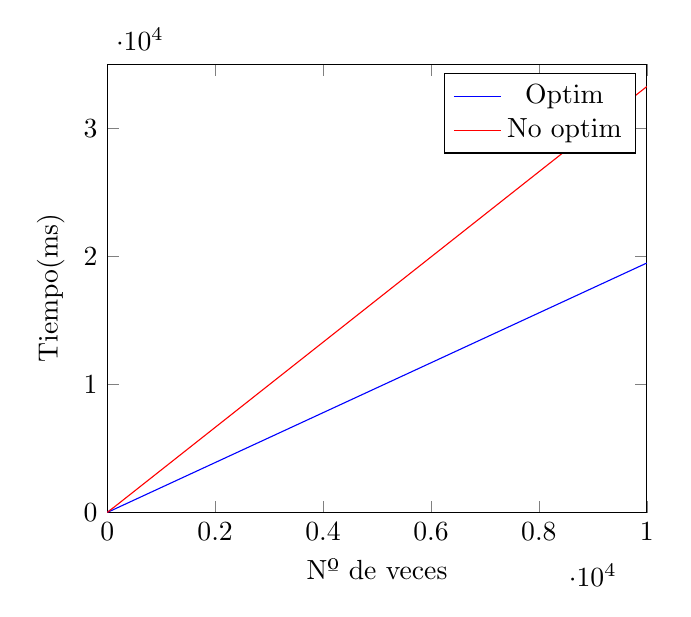
\begin{tikzpicture}
		\begin{axis}
			[ymin=0,ymax=35000, 
			xmin=0,xmax=10000, 
			ylabel= Tiempo(ms), 
			xlabel= Nº de veces] 
			\addplot+[smooth, mark=none] coordinates 
			{(1,2) (10,32) (100,196) (1000,1949) (10000,19479)};
			\addplot+[smooth, mark=none] coordinates
			{(1,3) (10,34) (100,332) (1000,3317) (10000,33256)};
			\legend{Optim, No optim}
		\end{axis}
	\end{tikzpicture}
	\caption{Comparación de optimización vs sin optimización. Segundo intento.}
\end{figure}

El resultado es claro, en cualquier caso acceder a la memoria de forma desordenada es un 50\% más costoso en este test. Por lo que la deducción es que hay que intentar mantener la memoria ordenada para una mayor eficiencia del programa. 
\\
Un apunte final que me veo obligado a hacer es que, tanto con el compilador de clang++, como el de g++, no hay que usar el flag ``-O3''. De ser así, al ser un test tan simple, el compilador es capaz de optimizar el código máquina y los resultados de ambos test son los mismos.

\section{Aprendizaje aleatorio vs \textit{backpropagation}}
\label{aleatorio vs backpropagation resultados}
Como quiero comparar las ventajas de usar \textit{backpropagation}, lo voy a hacer contra el algoritmo más sencillo, el que tenía inicialmente, que es el algoritmo aleatorio explicado en la figura \ref{Algoritmo aleatorio}. El problema que se tratará de resolver con el algoritmo es el de la XOR, y la arquitectura que va a tener la red neuronal es dos neuronas de entrada, una capa oculta con cuatro neuronas, y una neurona de salida que dice si la entrada ha producido verdadero o falso. 
\\
Como se puede apreciar en la siguiente figura, la linea roja representa el error que tiene la red cada 10 iteraciones, y la linea azul representa cómo va mejorando el error cuando el algoritmo se guarda el mejor resultado hasta el momento. Hay que tener en cuenta que, al ser cuatro soluciones las que tiene que dar (falso y falso, falso y verdadero, verdadero y falso, verdadero y verdadero), pero hay que representar el verdadero y el false numéricamente para calcular el error de la red, un error menor al 25\% significa que ha ajustado los pesos de la red para que los cuatro casos coincidan con la solución.
\begin{figure}[H]
	\centering
	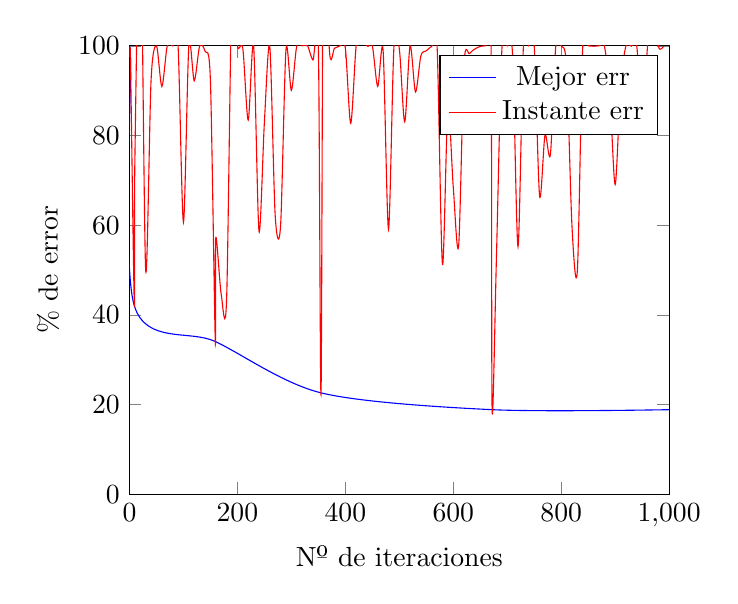
\begin{tikzpicture}
		\begin{axis}
			[ymin=0,ymax=100, 
			xmin=0,xmax=1000, 
			ylabel= \% de error, 
			xlabel= Nº de iteraciones] 
			\addplot+[smooth, mark=none] coordinates 
			{(0,99.8454) (1,97.5228) (2,95.9093) (9,42.0106) (159,34.0462) (355,22.5898) (672,18.837) (1000,18.837)};
			\addplot+[smooth, mark=none] coordinates
			{(0,99.8454) (1,97.5228) (2,95.9093) (9,42.0106) (10,74.5026)  (20,133.048) (30,50.0229) (40,92.3021) (50,100.001) (60,90.9467) (70,99.9676) (80,99.999) (90,99.994) (100,60.6559) (110,99.9855) (120,92.1943) (130,99.9257) (140,98.7933) (150,92.1119) (159,34.0462) (160,57.2305) (170,44.5407) (180,43.5673) (190,113.788) (200,100) (210,99.4142) (220,83.4381) (230,100.071) (240,58.6687) (250,82.9632) (260,99.8364) (270,62.1711) (280,59.9009) (290,99.1347) (300,90.076) (310,100) (320,99.984) (330,99.9887) (340,96.8439) (350,99.8101) (355,22.5898) (360,147.47) (370,100) (380,99.4627) (390,99.9865) (400,99.528) (410,82.7241) (420,99.9637) (430,104.989) (440,99.9984) (450,99.988) (460,90.9419) (470,98.9157) (480,59.0847) (490,99.6393) (500,99.3816) (510,83.033) (520,100) (530,89.7185) (540,97.7787) (550,98.865) (560,99.872) (570,99.9869) (580,51.2202) (590,85.9898) (600,68.4817) (610,55.4502) (620,95.9602) (630,98.2658) (640,99.2841) (650,99.8679) (660,99.999) (670,99.9999) (672,18.837) (680,52.8244) (690,98.9702) (700,99.9932) (710,97.9063) (720,55.2218) (730,99.942) (740,99.9992) (750,99.9678) (760,66.4945) (770,80.0553) (780,75.8166) (790,100.012) (800,99.9916) (810,95.3353) (820,59.7116) (830,49.9807) (840,99.9995) (850,99.9919) (860,99.9067) (870,99.9991) (880,99.9417) (890,89.8568) (900,69.0741) (910,91.0636) (920,99.9952) (930,99.9321) (940,100) (950,83.0578) (960,99.9856) (970,112.699) (980,99.9977) (990,100)};
			\legend{Mejor err, Instante err}
		\end{axis}
	\end{tikzpicture}
	\caption{Resultados del aprendizaje con un algoritmo aleatorio.}
\end{figure}

Otro dato interesante a conocer es en qué iteración el algoritmo encuentra una solución válida para resolver la XOR. El algoritmo itera 1000 veces. Después de ejecutar el algoritmo durante 10000 intentos, llego a la conclusión empírica de que el algoritmo encuentra una solución en la iteración 354.16 de media, siempre que lo encuentra. Sin embargo, hay un 19.83\% de las veces que el algoritmo aleatorio no es capaz de encontrar la solución. 
\\
Y no sólo vamos a fijarnos en el número de iteraciones que necesita el algoritmo, sino también en el tiempo, para después poder comparar con cuánto tiempo tarda contra \textit{backpropagation}. El algoritmo aleatorio tarda 12 segundos, en entrenar 10000 veces en mi máquina con optimizaciones, lo que quiere decir que de media tarda 0.0012 segundos en resolver el problema.

\begin{figure}[H]
	\centering
	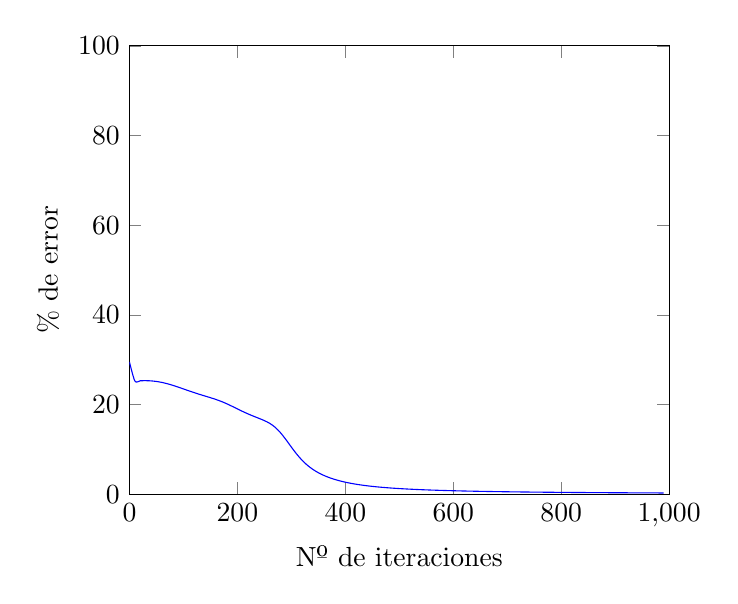
\begin{tikzpicture}
		\begin{axis}
			[ymin=0,ymax=100, 
			xmin=0,xmax=1000, 
			ylabel= \% de error, 
			xlabel= Nº de iteraciones] 
			\addplot+[smooth, mark=none] coordinates 
			{(0,29.4812) (10,25.2339) (20,25.2867) (30,25.3076) (40,25.2606) (50,25.1305) (60,24.9177) (70,24.63) (80,24.28) (90,23.8848) (100,23.4652) (110,23.0428) (120,22.6349) (130,22.2486) (140,21.8801) (150,21.5146) (160,21.1258) (170,20.6836) (180,20.1719) (190,19.6021) (200,19.0071) (210,18.4247) (220,17.8803) (230,17.3789) (240,16.9021) (250,16.4006) (260,15.7806) (270,14.905) (280,13.6765) (290,12.1482) (300,10.4941) (310,08.91017) (320,07.5336) (330,06.40639) (340,05.50272) (350,04.77621) (360,04.18526) (370,03.69856) (380,03.2934) (390,02.95306) (400,02.66494) (410,02.41928) (420,02.20841) (430,02.02622) (440,01.86781) (450,01.72924) (460,01.60728) (470,01.49934) (480,01.40327) (490,01.31734) (500,01.24009) (510,01.17033) (520,01.10706) (530,01.04946) (540,0.996808) (550,0.94853) (560,0.904119) (570,0.863146) (580,0.825243) (590,0.790093) (600,0.757419) (610,0.726983) (620,0.698574) (630,0.672007) (640,0.647119) (650,0.623765) (660,0.601818) (670,0.581161) (680,0.561692) (690,0.543317) (700,0.525955) (710,0.509528) (720,0.493969) (730,0.479216) (740,0.465212) (750,0.451905) (760,0.439248) (770,0.427198) (780,0.415716) (790,0.404765) (800,0.394311) (810,0.384324) (820,0.374776) (830,0.365639) (840,0.356891) (850,0.348507) (860,0.340468) (870,0.332753) (880,0.325345) (890,0.318227) (900,0.311384) (910,0.3048) (920,0.298463) (930,0.292358) (940,0.286476) (950,0.280803) (960,0.275331) (970,0.270048) (980,0.264947) (990,0.260017)};
		\end{axis}
	\end{tikzpicture}
	\caption{Resultados del aprendizaje con el algoritmo \textit{backpropagation}.}
	\label{Resultados XOR backpropagation}
\end{figure}

En la figura \ref{Resultados XOR backpropagation} se puede ver el número de iteraciones que hay que hacer para alcanzar una solución válida es mayor, con una estructura de la red neuronal equivalente (dos neuronas de entrada, una capa oculta con cuatro neuronas, y una neurona de salida).

De los 10.000 intentos de que el algoritmo solucione el problema en 1000 iteraciones,  se consigue el 96\% de las veces, a diferencia del 80,17\% que conseguía el algoritmo aleatorio. Mientras que el tiempo que tarda el algoritmo de \textit{backpropagation} es 12 segundos, es decir, el tiempo que tarda es equivalente. Por lo tanto se demuestra que \textit{backpropagation} tiene un mayor porcentaje de acierto. De media acierta en la iteración 426, esto significa que tarda más iteraciones, sin embargo, consigue un porcentaje de acierto más alto.

La gráfica \ref{Backpropagation cambiando learning rate} muestra, ya que \textit{backpropagation} tiene un parámetro para ajustar el ratio de aprendizaje, una comparación entre diferentes posibles valores del mismo. 
\begin{figure}[H]
	\centering
	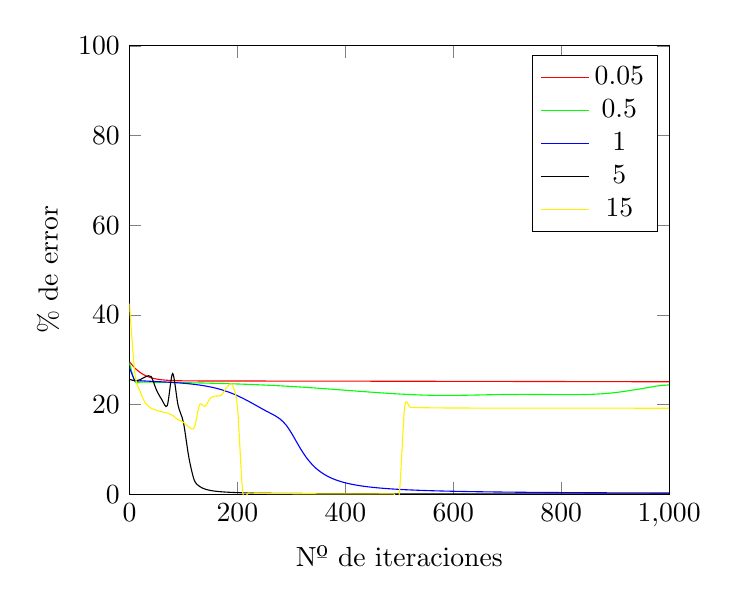
\begin{tikzpicture}
		\begin{axis}
			[ymin=0,ymax=100, 
			xmin=0,xmax=1000, 
			ylabel= \% de error, 
			xlabel= Nº de iteraciones] 
			\addplot+[smooth, mark=none, color=red] coordinates 
			{(0,29.512) (10,28.1277) (20,27.1086) (30,26.4112) (40,25.9586) (50,25.6752) (60,25.5017) (70,25.3968) (80,25.3338) (90,25.296) (100,25.2732) (110,25.2593) (120,25.2506) (130,25.245) (140,25.2412) (150,25.2385) (160,25.2364) (170,25.2346) (180,25.233) (190,25.2316) (200,25.2302) (210,25.2288) (220,25.2274) (230,25.226) (240,25.2246) (250,25.2232) (260,25.2218) (270,25.2203) (280,25.2188) (290,25.2173) (300,25.2158) (310,25.2143) (320,25.2127) (330,25.2111) (340,25.2095) (350,25.2079) (360,25.2062) (370,25.2046) (380,25.2029) (390,25.2011) (400,25.1994) (410,25.1976) (420,25.1959) (430,25.194) (440,25.1922) (450,25.1904) (460,25.1885) (470,25.1866) (480,25.1847) (490,25.1828) (500,25.1808) (510,25.1789) (520,25.1769) (530,25.1749) (540,25.1728) (550,25.1708) (560,25.1687) (570,25.1666) (580,25.1645) (590,25.1624) (600,25.1602) (610,25.1581) (620,25.1559) (630,25.1537) (640,25.1514) (650,25.1492) (660,25.1469) (670,25.1446) (680,25.1423) (690,25.14) (700,25.1377) (710,25.1353) (720,25.133) (730,25.1306) (740,25.1282) (750,25.1257) (760,25.1233) (770,25.1209) (780,25.1184) (790,25.1159) (800,25.1134) (810,25.1109) (820,25.1083) (830,25.1058) (840,25.1032) (850,25.1006) (860,25.098) (870,25.0954) (880,25.0927) (890,25.0901) (900,25.0874) (910,25.0848) (920,25.0821) (930,25.0794) (940,25.0766) (950,25.0739) (960,25.0711) (970,25.0684) (980,25.0656) (1000,25.0628)};
			\addplot+[smooth, mark=none, color=green] coordinates 
			{(0,29.3) (10,25.0566) (20,25.0105) (30,24.9931) (40,24.9757) (50,24.9583) (60,24.9408) (70,24.9229) (80,24.9045) (90,24.8853) (100,24.8651) (110,24.8438) (120,24.8211) (130,24.7969) (140,24.771) (150,24.7431) (160,24.7133) (170,24.6812) (180,24.6469) (190,24.6101) (200,24.5708) (210,24.5288) (220,24.4839) (230,24.4362) (240,24.3855) (250,24.3317) (260,24.2747) (270,24.2146) (280,24.1512) (290,24.0846) (300,24.0148) (310,23.942) (320,23.8661) (330,23.7874) (340,23.706) (350,23.6222) (360,23.5363) (370,23.4484) (380,23.3591) (390,23.2686) (400,23.1774) (410,23.0858) (420,22.9944) (430,22.9037) (440,22.8142) (450,22.7264) (460,22.6408) (470,22.5582) (480,22.479) (490,22.4039) (500,22.3336) (510,22.2686) (520,22.2098) (530,22.1577) (540,22.113) (550,22.0762) (560,22.0479) (570,22.0285) (580,22.0179) (590,22.0159) (600,22.0221) (610,22.0353) (620,22.0543) (630,22.0773) (640,22.1026) (650,22.1284) (660,22.1531) (670,22.1756) (680,22.195) (690,22.2107) (700,22.2226) (710,22.2307) (720,22.2353) (730,22.2368) (740,22.2355) (750,22.2319) (760,22.2266) (770,22.22) (780,22.2129) (790,22.2058) (800,22.1999) (810,22.1961) (820,22.1962) (830,22.202) (840,22.2161) (850,22.2416) (860,22.282) (870,22.3408) (880,22.4211) (890,22.5251) (900,22.6531) (910,22.8037) (920,22.9734) (930,23.1577) (940,23.3517) (950,23.5513) (960,23.7536) (970,23.9572) (980,24.1618) (1000,24.3679)};
			\addplot+[smooth, mark=none, color=blue] coordinates 
			{(0,28.248) (10,25.3732) (20,25.2915) (30,25.2241) (40,25.1636) (50,25.106) (60,25.0469) (70,24.9828) (80,24.9108) (90,24.8282) (100,24.7322) (110,24.6193) (120,24.4855) (130,24.3261) (140,24.1353) (150,23.9066) (160,23.6327) (170,23.3063) (180,22.9209) (190,22.472) (200,21.9589) (210,21.3852) (220,20.76) (230,20.0981) (240,19.4208) (250,18.7547) (260,18.1179) (270,17.4745) (280,16.668) (290,15.4365) (300,13.6576) (310,11.5672) (320,9.54095) (330,7.80622) (340,6.41307) (350,5.32242) (360,4.47286) (370,3.80792) (380,3.28268) (390,2.86313) (400,2.52397) (410,2.24648) (420,2.01678) (430,1.82452) (440,1.66192) (450,1.52308) (460,1.40347) (470,1.29961) (480,1.20875) (490,1.12873) (500,1.05781) (510,0.99461) (520,0.937991) (530,0.887026) (540,0.840947) (550,0.799118) (560,0.761003) (570,0.726151) (580,0.694179) (590,0.664761) (600,0.637618) (610,0.612507) (620,0.58922) (630,0.567575) (640,0.547413) (650,0.528595) (660,0.511) (670,0.494518) (680,0.479055) (690,0.464524) (700,0.450851) (710,0.437968) (720,0.425814) (730,0.414336) (740,0.403484) (750,0.393213) (760,0.383486) (770,0.374266) (780,0.36552) (790,0.357219) (800,0.349336) (810,0.341849) (820,0.334734) (830,0.327972) (840,0.321545) (850,0.315437) (860,0.309633) (870,0.304121) (880,0.298888) (890,0.293925) (900,0.28922) (910,0.284768) (920,0.280559) (930,0.276588) (940,0.27285) (950,0.269339) (960,0.266052) (970,0.262985) (980,0.260136) (1000,0.257503)};
			\addplot+[smooth, mark=none, color=black] coordinates 
			{(0,25.6122) (10,25.2806) (20,25.5486) (30,26.1927) (40,26.2346) (50,23.2293) (60,21.0663) (70,19.7438) (80,26.8959) (90,19.8321) (100,15.9827) (110,8.20897) (120,3.12829) (130,1.71361) (140,1.12593) (150,0.824623) (160,0.644778) (170,0.526445) (180,0.443183) (190,0.381668) (200,0.334504) (210,0.297276) (220,0.267194) (230,0.242415) (240,0.221673) (250,0.204072) (260,0.18896) (270,0.175852) (280,0.16438) (290,0.154262) (300,0.145274) (310,0.137241) (320,0.130019) (330,0.123495) (340,0.117572) (350,0.112173) (360,0.107232) (370,0.102695) (380,0.0985132) (390,0.0946486) (400,0.0910663) (410,0.0877371) (420,0.0846355) (430,0.0817391) (440,0.0790285) (450,0.0764867) (460,0.0740986) (470,0.0718509) (480,0.0697316) (490,0.0677303) (500,0.0658374) (510,0.0640446) (520,0.0623441) (530,0.0607292) (540,0.0591936) (550,0.0577316) (560,0.0563383) (570,0.0550088) (580,0.053739) (590,0.0525251) (600,0.0513633) (610,0.0502506) (620,0.0491838) (630,0.0481603) (640,0.0471775) (650,0.0462329) (660,0.0453246) (670,0.0444504) (680,0.0436085) (690,0.0427971) (700,0.0420147) (710,0.0412597) (720,0.0405307) (730,0.0398265) (740,0.0391458) (750,0.0384874) (760,0.0378503) (770,0.0372335) (780,0.036636) (790,0.036057) (800,0.0354956) (810,0.0349511) (820,0.0344226) (830,0.0339096) (840,0.0334113) (850,0.0329271) (860,0.0324565) (870,0.0319988) (880,0.0315537) (890,0.0311205) (900,0.0306988) (910,0.0302881) (920,0.0298881) (930,0.0294983) (940,0.0291183) (950,0.0287478) (960,0.0283865) (970,0.0280339) (980,0.0276899) (1000,0.027354)};
			\addplot+[smooth, mark=none, color=yellow] coordinates 
			{(0,42.4898) (10,26.8803) (20,22.8098) (30,20.214) (40,19.1996) (50,18.6843) (60,18.3622) (70,18.0976) (80,17.5636) (90,16.6035) (100,16.0297) (110,14.9599) (120,14.8262) (130,19.9627) (140,19.5791) (150,21.4538) (160,21.875) (170,22.0504) (180,23.7649) (190,24.4441) (200,19.458) (210,0.317342) (220,0.254418) (230,0.212609) (240,0.18255) (250,0.159892) (260,0.142216) (270,0.128057) (280,0.116475) (290,0.106839) (300,0.0987078) (310,0.0917677) (320,0.0857866) (330,0.0805911) (340,0.0760492) (350,0.0720591) (360,0.0685418) (370,0.0654361) (380,0.0626946) (390,0.0602823) (400,0.0581747) (410,0.0563583) (420,0.0548319) (430,0.05361) (440,0.0527314) (450,0.0522758) (460,0.0524051) (470,0.0534717) (480,0.0563899) (490,0.0645567) (500,0.117378) (510,19.4729) (520,19.3731) (530,19.3201) (540,19.2874) (550,19.2651) (560,19.2491) (570,19.2369) (580,19.2275) (590,19.2199) (600,19.2136) (610,19.2085) (620,19.2041) (630,19.2003) (640,19.1971) (650,19.1943) (660,19.1918) (670,19.1896) (680,19.1876) (690,19.1858) (700,19.1842) (710,19.1828) (720,19.1815) (730,19.1803) (740,19.1792) (750,19.1782) (760,19.1773) (770,19.1764) (780,19.1757) (790,19.1749) (800,19.1742) (810,19.1736) (820,19.173) (830,19.1725) (840,19.172) (850,19.1715) (860,19.1711) (870,19.1706) (880,19.1703) (890,19.1699) (900,19.1695) (910,19.1692) (920,19.1689) (930,19.1686) (940,19.1684) (950,19.1681) (960,19.1679) (970,19.1677) (980,19.1675) (1000,19.1673)};
			\legend{0.05, 0.5, 1, 5, 15}
		\end{axis}
	\end{tikzpicture}
	\caption{Resultados del aprendizaje con el algoritmo \textit{backpropagation}, según el learning rate.}
	\label{Backpropagation cambiando learning rate}
\end{figure}

Se aprecia que ratios de aprendizaje extremadamente bajos y extremadamente altos hacen que la red no aprenda bien, por diferentes motivos. No se puede decir un ratio que sea común para todos los problemas, por eso en el juego dejo experimentar al usuario con distintos ratios para que encuentre el mejor. 

\section{\textit{Backpropagation} en el juego}
Como ya he comentado, he tenido problemas en el aprendizaje dentro del juego. La red neuronal no aprendía tan bien como en el problema de la XOR, y finalmente descubrí que era a causa, entre otras cosas, del \textit{learning rate} mayormente. Y como se puede ver en la figura \ref{error erratico}, valores cercanos a uno provocan que la red no sea capaz de aprender. Pero depurando más profundamente, detecto lo que puede ser la explicación al error.

Con una arquitectura de la red de 16 entradas, una capa intermedia de 4 neuronas y 2 salidas, para un valor de \textit{learning rate} alto (cercano a uno) sucede lo que se puede ver en la figura \ref{alto learning rate arquitectura simple}. Los pesos de la primera capa (la que conecta las 16 neuronas con las 4) mantienen los valores obtenidos aleatoriamente, no varían en todo el entrenamiento, mientras que los de la segunda capa (la que conecta las 4 neuronas con las 2 de salida) sí que lo hacen. Sin embargo, si uso un ratio de aprendizaje menor a 0.001, ambas capas de pesos cambian, pero sigo sin conseguir un resultado satisfactorio, una arquitectura tan simple no es capaz de aprender a jugar, pero sí que varían los parámetros de la primera capa.

\begin{figure}[H]
	\centering
	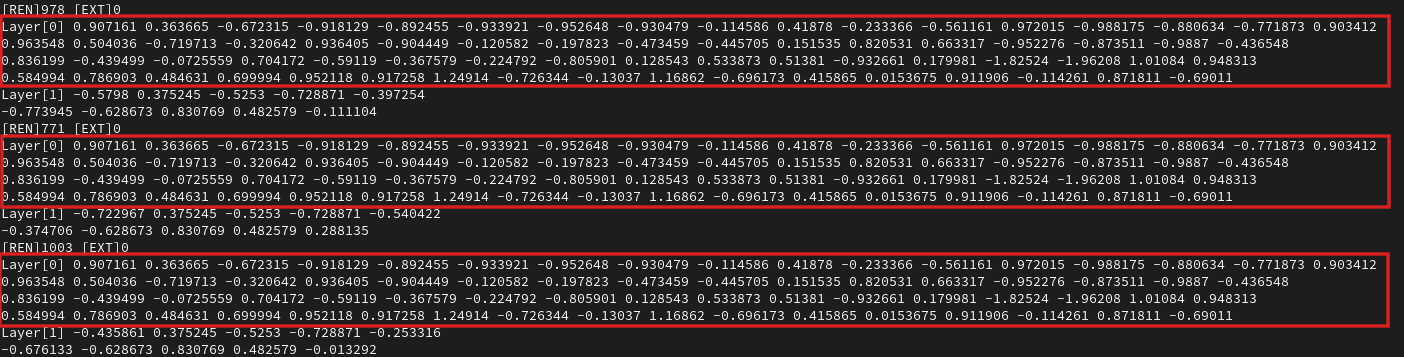
\includegraphics[width=15cm]{archivos/imagenes/alto-learning-rate-arquitectura-simple.png}
	\caption{Varianza de peso en arquitectura simple con un learning rate alto.}
	\label{alto learning rate arquitectura simple}
\end{figure}

Ahora pruebo con una arquitectura más compleja, 16 neuronas de entrada, 4 capas ocultas de 6 neuronas cada una, y 2 neuronas de salida. Además un total de 10000 iteraciones, y la distribución de la muestra es aproximadamente 40\% muestras de tocar arriba, 40\% muestras de tocar abajo, y 20\% muestras de no tocar. Para valores cercanos a uno sigue sucediendo lo visto en la figura \ref{error erratico}, y además, sucede lo mismo que en la figura \ref{alto learning rate arquitectura simple}, que la primera capa no varía, mientras que el resto sí que lo hace. Sin embargo, para un valor del ratio de aprendizaje menor a 0.001, la red si que aprende y sucede lo que puedes ver en la figura \ref{error concordante}, obtenemos errores bajos corregidos a lo largo de las 10000 iteraciones en los tres gráficos, y cuando ponemos la red resultante a jugar, lo hace de manera satisfactoria. 

\begin{figure}[H]
	\centering
	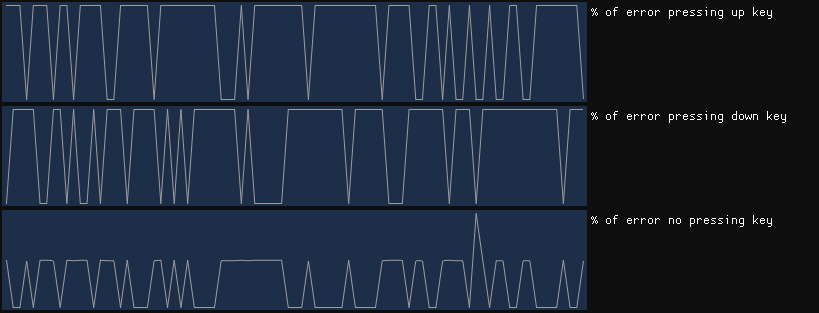
\includegraphics[width=15cm]{archivos/imagenes/arquitectura-compleja-learning-rate-alto.png}
	\caption{Porcentaje de acierto con arquitectura compleja y learning rate alto.}
	\label{alto learning rate arquitectura compleja}
\end{figure}

Por último, pongo a entrenar a la red más compleja que permite el juego. Será una arquitectura de 16 neuronas de entrada, 10 capas ocultas con 10 neuronas cada una, y con 2 neuronas de salida.  Diez mil iteraciones como antes, y un ratio de aprendizaje del 0.743. Lo que pasa en este caso es que, sorprendentemente, cambian todos los pesos de todas las capas (incluida la primera capa), pero las últimas capas cambian mucho más rápido que las primeras (como ha sucedido también en los anteriores ejemplos). Los resultados de las gráficas son muy parecidos a los ya comentados antes con learning rate alto, pero he tomado otra captura que puedes ver en la figura \ref{alto learning rate arquitectura compleja} para dejarlo demostrado.

Lo siguiente que hago es poner a entrenar la misma arquitectura, pero con un learning rate de 0.0074 durante diez mil iteraciones, y una distribución de los datos 40-40-20 como ya he comentado antes. Todos los pesos  de todas las capas están variando, pero con una velocidad de cambio menor. El resultado final de esta red tan compleja es el que se puede ver en la figura \ref{bajo learning rate arquitectura compleja}, \textit{backpropagation} no es capaz de corregir el error con este número de iteraciones, y lo más normal será que se quede con un 0\% de error ``no pulsar'' y 100\% ``pulsar'', porque al generar la red de manera aleatoria, es lo más probable. Los resultados son los mismos con un valor de learning rate intermedio como 0.359.
\begin{figure}[H]
	\centering
	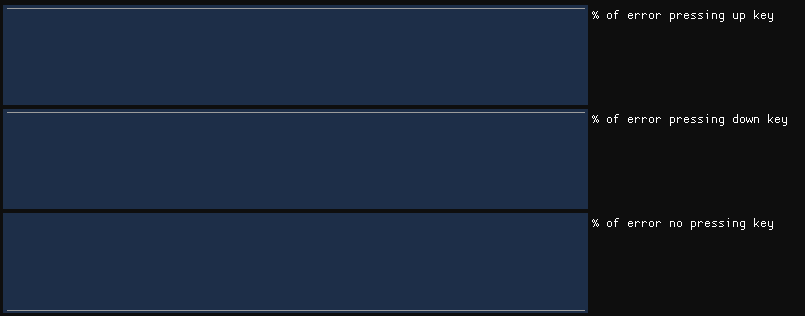
\includegraphics[width=15cm]{archivos/imagenes/arquitectura-compleja-learning-rate-bajo.png}
	\caption{Porcentaje de acierto con arquitectura compleja y learning rate bajo.}
	\label{bajo learning rate arquitectura compleja}
\end{figure}

En última instancia he querido comprobar si la red se comportaba mejor con un número menor de entradas. En principio esto no debería afectar mucho según la teoría de la dimensión Vapnik-Chervonenkis porque el número de términos independientes es prácticamente el mismo, sin embargo, los resultados no dicen lo mismo. Los datos que se le pasan a la red original del juego son, la posición x e y, velocidades x e y, y la aceleración tanto del agente, como de las pelotas, como del minion mas cercano. La aceleración sólo al minion y el agente, que son los que la aplican al pulsar para moverse.
\\
El primer intento fue quitar la aceleración como entrada, comprobé que durante el entrenamiento se cometía menos fallos, pero a la hora de jugar era similar. El segundo intento fue quitar también los valores del minion, mismo resultado que al principio. Y por último decidí dejar sólo como entrada la posición x e y del agente y las dos pelotas. En este último intento sí que noté algo de mejoría en la forma de jugar, el agente había aprendido a jugar casi tan acertado como cuando solo había dos perceptrones. Y aunque el número de términos independientes sea prácticamente el mismo, sí que hay una explicación para este suceso: el agente aprende mejor porque las posiciones x e y son los datos más relevantes de la muestra, aunque se puede extraer información interesante del resto de datos, el agente será capaz de extraer más fácilmente el ruido de la muestra si sólo pongo los datos más relevantes como entradas a la red.